\begin{frame}[fragile]
\frametitle{Aufbau und Modell}

\begin{center}
		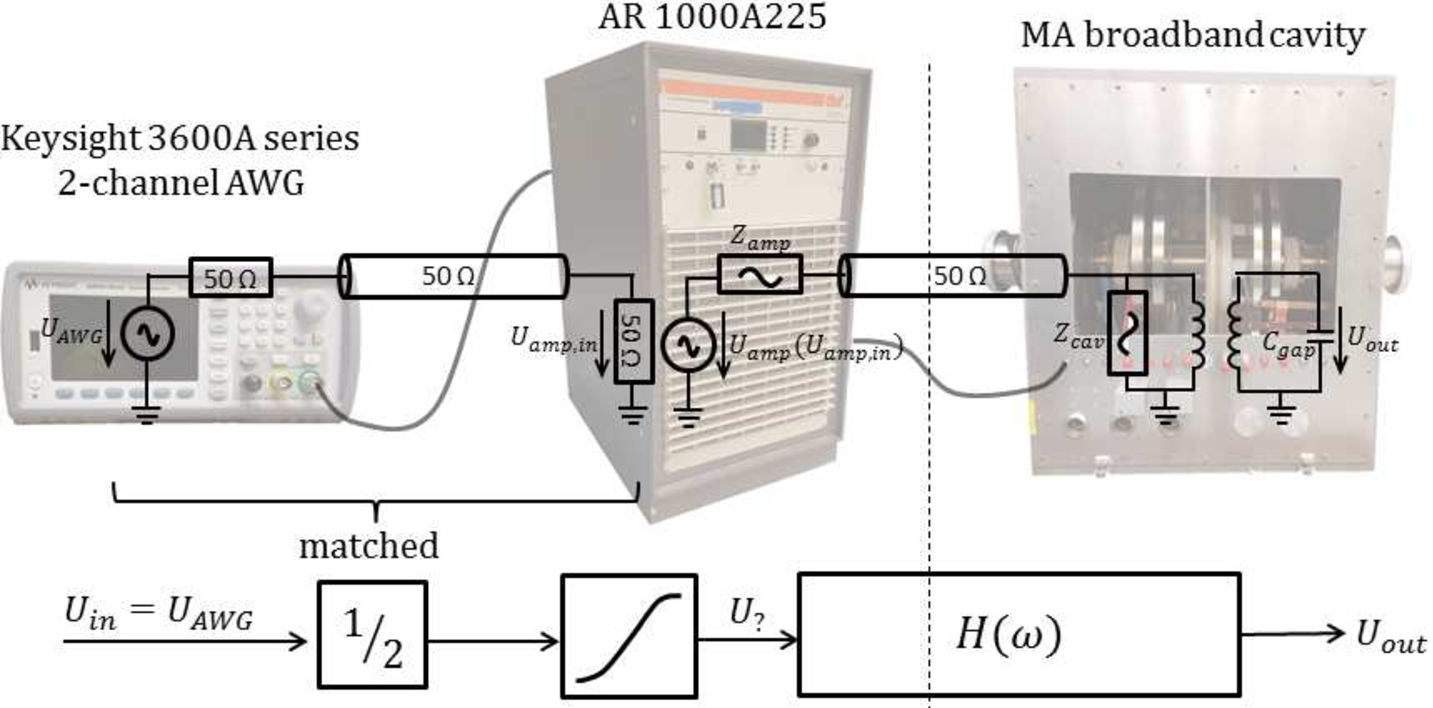
\includegraphics[scale=0.45]{slides/ResultCode/WEPVA047f2_2-eps-converted-to.pdf} 
	\end{center}
\end{frame}

\begin{frame}[fragile]
\frametitle{Aufbau und Modell}

	
	{
	\begin{itemize}
	\uncover<2->{
	\item Gegeben:
		\begin{itemize} 
			\item Lineare Übertragungsfunktion $H$ bestimmt durch Pseudorauschen
			\item System linear bis $\hat{U}_{BB} \approx 550V$ genähert
		\end{itemize}
		}
		\uncover<3->{
	\item Hammerstein Modell : 
		\begin{itemize}
			\item Ergänzung um eine nichtlineare Vorverzerrung mit einem Potenzreihenansatz 
		\end{itemize}
		\begin{center}
		%\begin{align*}
		$	U_?(t)=\sum_{n=1}^N \, a_n \, \left[ U_{in}(t) \right]^n
			\quad
			\underline{U}_{out} \left( \omega \right) = H \left( \omega \right) \cdot \underline{U}_{?} \left( \omega \right)
		$\\		
		%\end{align*}
		}
		\end{center}
		\uncover<4->{
	\item Zielsetzung :
		\begin{itemize}
			\item Parameter $a_n$ der Kennlinie $K$ zubestimmen
			\item Ersten Optimierungs Ansatz implementieren
		\end{itemize}
		}	
	 \end{itemize}
	
	\centering
	\begin{picture}(100,70)
		\put(15,5){
			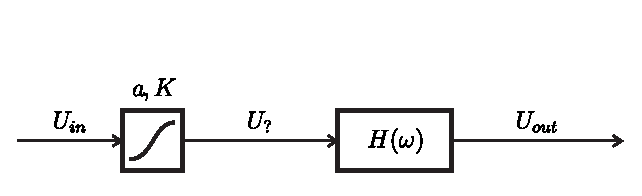
\includegraphics[scale=1.0]{slides/Problemstellung/Slide1.eps} 
		}
	\end{picture}
	}
%\begin{picture}(100,70)
%		\put(15,0){
%			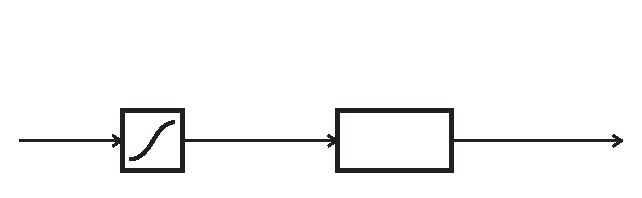
\includegraphics[scale=1.0]{slides/ResultCode/Slide2.eps} 
%		}  
%	\end{picture}
\end{frame}
